\documentclass[12pt,letterpaper]{article}
\usepackage{apa_manual}
\apatituloCorto{Modelos clásicos y Machine Learning}

\begin{document}

\apacabecera
  {Modelos clásicos de referencia y aprendizaje automático en revisiones del PBI}
  {Manual teórico y práctico 5 — Fundamento completo de la Etapa 3}
  {Para saber si una arquitectura cuántica aporta verdadero valor predictivo, primero debemos medir con rigor qué tan bien funcionan las herramientas estadísticas y de Machine Learning ya establecidas. Este manual explica las \(20\) variables de entrada disponibles en tiempo real, las ecuaciones y mecanismos de los ocho modelos de referencia de la Etapa~3, su desempeño real por regímenes y la lección crítica que dejó el choque del COVID-19.}

\section{El tablero común: los 20 predictores observables en tiempo real}

En las Etapas~3 y~5 evaluamos ocho especificaciones en estricto tiempo real sobre \(n = 250\) orígenes fuera de muestra comprendidos entre febrero de 2003 (\codigo{2003m2}, cuando ya existen \(90\) revisiones limpias completadas para entrenar) y noviembre de 2024 (\codigo{2024m11}, con \(339\) observaciones completadas en la última ventana). Reservamos además los últimos \(60\) meses (\texttt{2019m12}--\texttt{2024m11}) como \emph{bloque congelado final} que no se utilizó para diseñar arquitecturas.

Todos los modelos multivariados consumen exactamente la misma matriz causal \(\mathbf{x}_t \in \mathbb{R}^{20}\) construida por \codigo{build\_realtime\_feature\_table} en \codigo{scripts/rtd\_eval\_utils.py}, cuyos \(20\) predictores observables en \(v_0(t)\) pertenecen a cinco bloques económicos:
\begin{enumerate}
  \item \textbf{Dinámica inmediata del PBI publicado en \(v_0(t)\) (3 variables):} primera estimación \codigo{y0} (\(y_t^{(v_0)}\)), cambio mensual reciente \codigo{dy0\_1m} (\(y_t^{(v_0)} - y_{t-1}^{(v_0)}\)) y promedio móvil trimestral \codigo{y0\_ma3} dentro del mismo boletín.
  \item \textbf{Desagregación sectorial instantánea (6 variables):} primeras tasas publicadas en \(v_0(t)\) de las seis ramas continuas (\codigo{sec\_agriculture}, \codigo{sec\_commerce}, \codigo{sec\_construction}, \codigo{sec\_fishing}, \codigo{sec\_manufacturing}, \codigo{sec\_mining}).
  \item \textbf{Memoria anual de revisiones ya finalizadas (4 variables):} los tres rezagos completados en o antes de \(v_0(t)\) (\codigo{Y\_lag11}, \codigo{Y\_lag12}, \codigo{Y\_lag13}) y el promedio de las seis últimas revisiones completadas (\codigo{Y\_obs\_mean6}).
  \item \textbf{Revisiones tempranas de corto plazo ya visibles en \(v_0(t)\) (3 variables):} correcciones acumuladas observadas hasta \(v_0(t)\) para los tres meses precedentes (\codigo{rev\_short\_s} \(= y_{t-s}^{(v_0(t))} - y_{t-s}^{(v_0(t-s))}\) para \(s \in \{1, 2, 3\}\), excluyendo cruces de año base).
  \item \textbf{Estacionalidad armónica del mes objetivo (4 variables):} pares trigonométricos de frecuencias anual y semestral (\(\sin_1, \cos_1, \sin_2, \cos_2\) de \(2\pi m_t / 12\) y \(4\pi m_t / 12\)) para capturar suavemente el ciclo estacional hallado en la Etapa~2 sin gastar \(11\) grados de libertad en variables ficticias.
\end{enumerate}

Toda imputación de valores faltantes (mediana) y estandarización (\(z\)-score) se estima exclusivamente dentro de cada ventana causal de entrenamiento antes de emitir la predicción del mes \(t\).

\section{Anatomía de las ocho especificaciones clásicas}

Cada modelo clásico responde a una pregunta económica concreta sobre la señal presente en las revisiones.

\subsection{Referencia nula y esquemas de corrección de sesgo}

Los tres referentes univariados más sencillos establecen el piso mínimo que cualquier modelo complejo debe superar:
\begin{itemize}
  \item \textbf{Referencia nula (\codigo{Zero}):} fija siempre \(\widehat{Y}_t = 0\). Mide directamente el error cuadrático que sufriría un analista que tratara cada primera publicación del BCRP como definitiva (hipótesis pura de \emph{News}).
  \item \textbf{Media expansiva (\codigo{BiasCorr\_Mean}):} pronostica \(\widehat{Y}_t = \bar{Y}_{\text{train}}\), el promedio aritmético de todas las revisiones pasadas ya concluidas. Corrige el sesgo positivo histórico sin usar covariables, pero arrastra con igual peso las revisiones grandes de los años noventa aun después de 2014.
  \item \textbf{Media móvil de 60 meses (\codigo{BiasCorr\_Roll60}):} calcula el promedio únicamente sobre las \(60\) revisiones completadas más recientes. Aunque sacrifica tamaño muestral, se adapta rápidamente cuando el sesgo cae tras el cambio de base de 2014.
\end{itemize}

\subsection{Modelos autorregresivos causales (AR\_BIC y ARX\_BIC)}

Para explotar la persistencia anual verificada en la Etapa~2 (\(\hat{\rho}_{12} = +0{,}386\)), \codigo{AR\_BIC} y \codigo{ARX\_BIC} estiman por mínimos cuadrados ordinarios la ecuación:
\begin{equation}
  \widehat{Y}_t = \hat{\alpha} + \sum_{k=1}^{p} \hat{\phi}_k\, Y_{t-10-k} + \underbrace{\hat{\gamma}_1 y_{0,t} + \hat{\gamma}_2 \sin\!\left(\tfrac{2\pi m_t}{12}\right) + \hat{\gamma}_3 \cos\!\left(\tfrac{2\pi m_t}{12}\right)}_{\text{Presente solo en ARX}},
  \label{eq:ar_arx}
\end{equation}
sobre los rezagos completados \(Y_{t-11}, Y_{t-12}, Y_{t-13}\). En cada mes \(t\), el orden \(p \in \{1, 2, 3\}\) se selecciona automáticamente sobre la muestra común de entrenamiento minimizando el criterio de información bayesiano \(\text{BIC} = n_c \ln(\hat{\sigma}^2) + k \ln(n_c)\). En la práctica, el algoritmo escogió \(p = 2\) (rezagos 11 y 12) en el \(99{,}2\%\) de los orígenes para \codigo{AR\_BIC} (\(248/250\)) y en el \(98{,}8\%\) para \codigo{ARX\_BIC} (\(247/250\)), reflejando exactamente la estructura temporal revelada por el correlograma.

\subsection{Regresión regularizada Ridge (benchmark principal) y DFM-PCA}

Cuando introducimos simultáneamente los \(20\) predictores de \(\mathbf{x}_t\) en una regresión lineal ordinaria (MCO), la fuerte colinealidad entre el PBI total (\codigo{y0}), su promedio móvil (\codigo{y0\_ma3}) y los seis sectores productivos dispara la varianza de los coeficientes estimados. La regresión \textbf{Ridge} \parencite{hoerl1970} —designada ex ante como nuestro benchmark lineal principal— resuelve esta inestabilidad agregando una penalización cuadrática \(L_2\) sobre los pesos (dejando libre el intercepto centrado \(\bar{Y}_{\text{tr}}\)):
\begin{equation}
  \hat{\beta}_{\text{Ridge}} = \arg\min_{\beta \in \mathbb{R}^{20}} \sum_{s \in \text{Train}} \bigl(Y_s - \bar{Y}_{\text{tr}} - \tilde{\mathbf{x}}_s^{\top}\beta\bigr)^2 + \lambda \sum_{j=1}^{20} \beta_j^2,
  \label{eq:ridge}
\end{equation}
cuya solución analítica cerrada es \(\hat{\beta}_{\text{Ridge}} = (\tilde{\mathbf{X}}_{\text{tr}}^{\top}\tilde{\mathbf{X}}_{\text{tr}} + \lambda I_{20})^{-1} \tilde{\mathbf{X}}_{\text{tr}}^{\top}(\mathbf{y}_{\text{tr}} - \bar{Y}_{\text{tr}})\). Para seleccionar \(\lambda\) sin mirar el futuro, el script \codigo{etapa3\_modelos\_clasicos.py} evalúa una grilla de diez valores \(\lambda \in \{0{,}5; 1; 2; 5; 10; 25; 50; 100; 250; 500\}\) mediante validación temporal causal sobre los últimos \(\min(36, \max(18, \lfloor n_{\text{tr}}/4\rfloor))\) puntos internos, acelerando el cálculo mediante una única descomposición en valores singulares (SVD) por ventana interna. Debido a la alta colinealidad sectorial, Ridge escogió el tope \(\lambda = 500\) en \(164/250\) orígenes (\(65{,}6\%\)).

Como alternativa parsimoniosa inspirada en la literatura de \emph{nowcasting} factorial \parencite{stock2002, giannone2008, banbura2011}, el modelo \textbf{DFM-PCA + Ridge} aplica primero SVD dentro de cada ventana de entrenamiento sobre las seis ramas sectoriales estandarizadas para extraer \(k = 2\) factores latentes comunes, los combina con seis variables centrales (\codigo{y0}, \codigo{Y\_lag11}, \codigo{Y\_lag12}, \codigo{Y\_obs\_mean6}, \(\sin_1, \cos_1\)) formando ocho regresores totales, y ajusta la Ecuación~\ref{eq:ridge} con \(\lambda \in [0{,}5;\; 100]\).

\subsection{Árboles impulsados por gradiente (GBDT\_NumPy)}

Mientras las ecuaciones anteriores asumen una superficie de respuesta lineal plana, los árboles impulsados por gradiente (\emph{Gradient Boosted Decision Trees}) \parencite{friedman2001} construyen una función escalonada no lineal sumando \(M\) árboles de regresión CART poco profundos, donde cada nuevo árbol \(T_m\) se entrena para reducir los pseudo-residuos \(r_s^{(m)} = Y_s - F_{m-1}(\mathbf{x}_s)\) dejados por el ensamble previo:
\begin{equation}
  \widehat{Y}_t = F_0 + \nu \sum_{m=1}^{M} T_m(\mathbf{x}_t),
  \label{eq:gbdt}
\end{equation}
partiendo de \(F_0 = \bar{Y}_{\text{tr}}\) y amortiguando cada paso con una tasa de aprendizaje pequeña \(\nu\). Dado que el paquete C++ \codigo{xgboost} no se encontraba instalado en el entorno Python del proyecto, implementamos una versión exacta y determinista en NumPy puro (\codigo{GBDT\_NumPy}): cada nodo elige el corte \(x_{s,j} \le \tau\) que maximiza la reducción cuadrática \(\frac{S_L^2}{n_L} + \frac{S_R^2}{n_R}\) sujeto a un mínimo de \(8\) observaciones por hoja (\texttt{min\_leaf = 8}), sintonizando trimestralmente por validación temporal interna la profundidad máxima \(d \in \{1, 2\}\), la tasa \(\nu \in \{0{,}03;\, 0{,}06\}\) y el número de árboles \(M \in \{25, 50\}\). En el \(55{,}6\%\) de los orígenes seleccionó \emph{stumps} de profundidad \(d = 1\) (y en \(72/250\) la terna más conservadora \(d=1, \nu=0{,}03, M=25\)).

\section{Resultados por regímenes y el mecanismo del colapso lineal en 2020--2021}

La Tabla~\ref{tab:etapa3_resumen} reúne las métricas exactas fuera de muestra de los ocho referentes clásicos en la muestra global (\(n=250\)) y desagregadas por subperíodos históricos y bloque congelado final. La lectura conjunta de estas columnas contiene el hallazgo metodológico más instructivo de la primera mitad del proyecto.

\begin{table}[htbp]
  \caption{Desempeño real fuera de muestra de los ocho referentes clásicos por régimen (Etapa~3)}
  \label{tab:etapa3_resumen}
  \centering
  \scriptsize
  \setlength{\tabcolsep}{3.0pt}
  \begin{tabular}{@{}p{3.2cm} S[table-format=1.3] S[table-format=1.3] S[table-format=-1.3] S[table-format=1.3] S[table-format=1.3] S[table-format=1.3] S[table-format=-1.3]@{}}
    \toprule
    & \multicolumn{3}{c}{Global (\(n=250\))} & {Pre-base} & {Pos-base} & \multicolumn{2}{c}{Congelado (\(n=60\))} \\
    \cmidrule(lr){2-4} \cmidrule(lr){5-5} \cmidrule(lr){6-6} \cmidrule(lr){7-8}
    Modelo & {RMSE} & {MAE} & {$R^2_{\text{OOS}}$} & {RMSE (\(119\))} & {RMSE (\(71\))} & {RMSE} & {$R^2_{\text{OOS}}$} \\
    \midrule
    \codigo{Zero} (\(\widehat{Y}=0\)) & 0.574 & 0.396 & -0.349 & 0.735 & 0.254 & 0.474 & -0.682 \\
    \codigo{BiasCorr\_Mean}           & 0.513 & 0.395 & -0.077 & 0.654 & 0.302 & 0.371 & -0.033 \\
    \codigo{BiasCorr\_Roll60}         & 0.525 & 0.381 & -0.127 & 0.688 & {\textbf{0,210}} & 0.396 & -0.175 \\
    \codigo{AR\_BIC}                  & 0.498 & {\textbf{0,356}} & -0.016 & 0.638 & 0.243 & 0.396 & -0.175 \\
    \codigo{ARX\_BIC}                 & 0.558 & 0.384 & -0.276 & 0.625 & 0.268 & 0.663 & -2.290 \\
    \codigo{Ridge} (benchmark)        & 0.566 & 0.384 & -0.312 & {\textbf{0,605}} & 0.251 & 0.731 & -3.001 \\
    \codigo{DFM\_Factor\_Ridge}       & 0.605 & 0.392 & -0.498 & 0.617 & 0.266 & 0.827 & -4.125 \\
    \codigo{GBDT\_NumPy}              & {\textbf{0,495}} & {\textbf{0,356}} & -0.003 & 0.646 & 0.245 & {\textbf{0,349}} & {\textbf{+0,087}} \\
    \bottomrule
  \end{tabular}
  \apanota{Datos verificados en \codigo{output/etapa3\_clasicos/etapa3\_metricas\_globales.csv} y \codigo{etapa3\_metricas\_subperiodos.csv}. En negrita se destaca el mejor desempeño de cada columna.}
\end{table}

Al analizar la Tabla~\ref{tab:etapa3_resumen} por períodos, emergen tres fenómenos complementarios:
\begin{enumerate}
  \item \textbf{Superioridad de Ridge en tiempos normales:} en el tramo pre-base (\texttt{2003m2}--\texttt{2013m2}, \(n=119\)) y en todo el bloque pre-COVID combinado (\texttt{2003m2}--\texttt{2019m11}, \(n=190\)), \codigo{Ridge} encabeza la competencia clásica con \(\text{RMSE} = 0{,}503\) y \(R^2_{\text{OOS}} = +0{,}094\), superando de manera estadísticamente significativa tanto a \codigo{BiasCorr\_Mean} (\(\text{RMSE} = 0{,}550\), \(p_{\text{DM}} = 0{,}0071\)) como a \codigo{GBDT\_NumPy} (\(\text{RMSE} = 0{,}533\), \(p_{\text{DM}} = 0{,}0086\)). Esto confirma que, en régimen estacionario, las relaciones con las variables observables son esencialmente lineales y los árboles CART pierden algo de eficiencia al discretizar fronteras continuas.
  \item \textbf{Adaptación rápida tras el cambio de base de 2014:} en el régimen calmo pos-2014 (\texttt{2014m1}--\texttt{2019m11}, \(n=71\)), donde la revisión media descendió a \(+0{,}163\) p.p., la media móvil de \(60\) meses (\codigo{BiasCorr\_Roll60}) obtiene el mínimo error (\(\text{RMSE} = 0{,}210\), sesgo \(+0{,}003\)), mientras \codigo{BiasCorr\_Mean} empeora (\(\text{RMSE} = 0{,}302\)) por seguir promediando las revisiones más altas de 1994--2012.
  \item \textbf{El desastre de la extrapolación lineal durante el COVID-19:} en el bloque congelado final (\(n=60\)), todos los modelos lineales que incluyen \(y_0\) o combinaciones lineales sectoriales sin cota sufren un colapso severo (\codigo{ARX\_BIC} \(\text{RMSE}=0{,}663\), \codigo{Ridge} \(0{,}731\), \codigo{DFM\_Factor\_Ridge} \(0{,}827\)).
\end{enumerate}

\begin{figure}[htbp]
  \caption{Extrapolación lineal de Ridge frente a saturación acotada de GBDT durante el choque COVID-19}
  \label{fig:ridge_gbdt_covid}
  \centering
  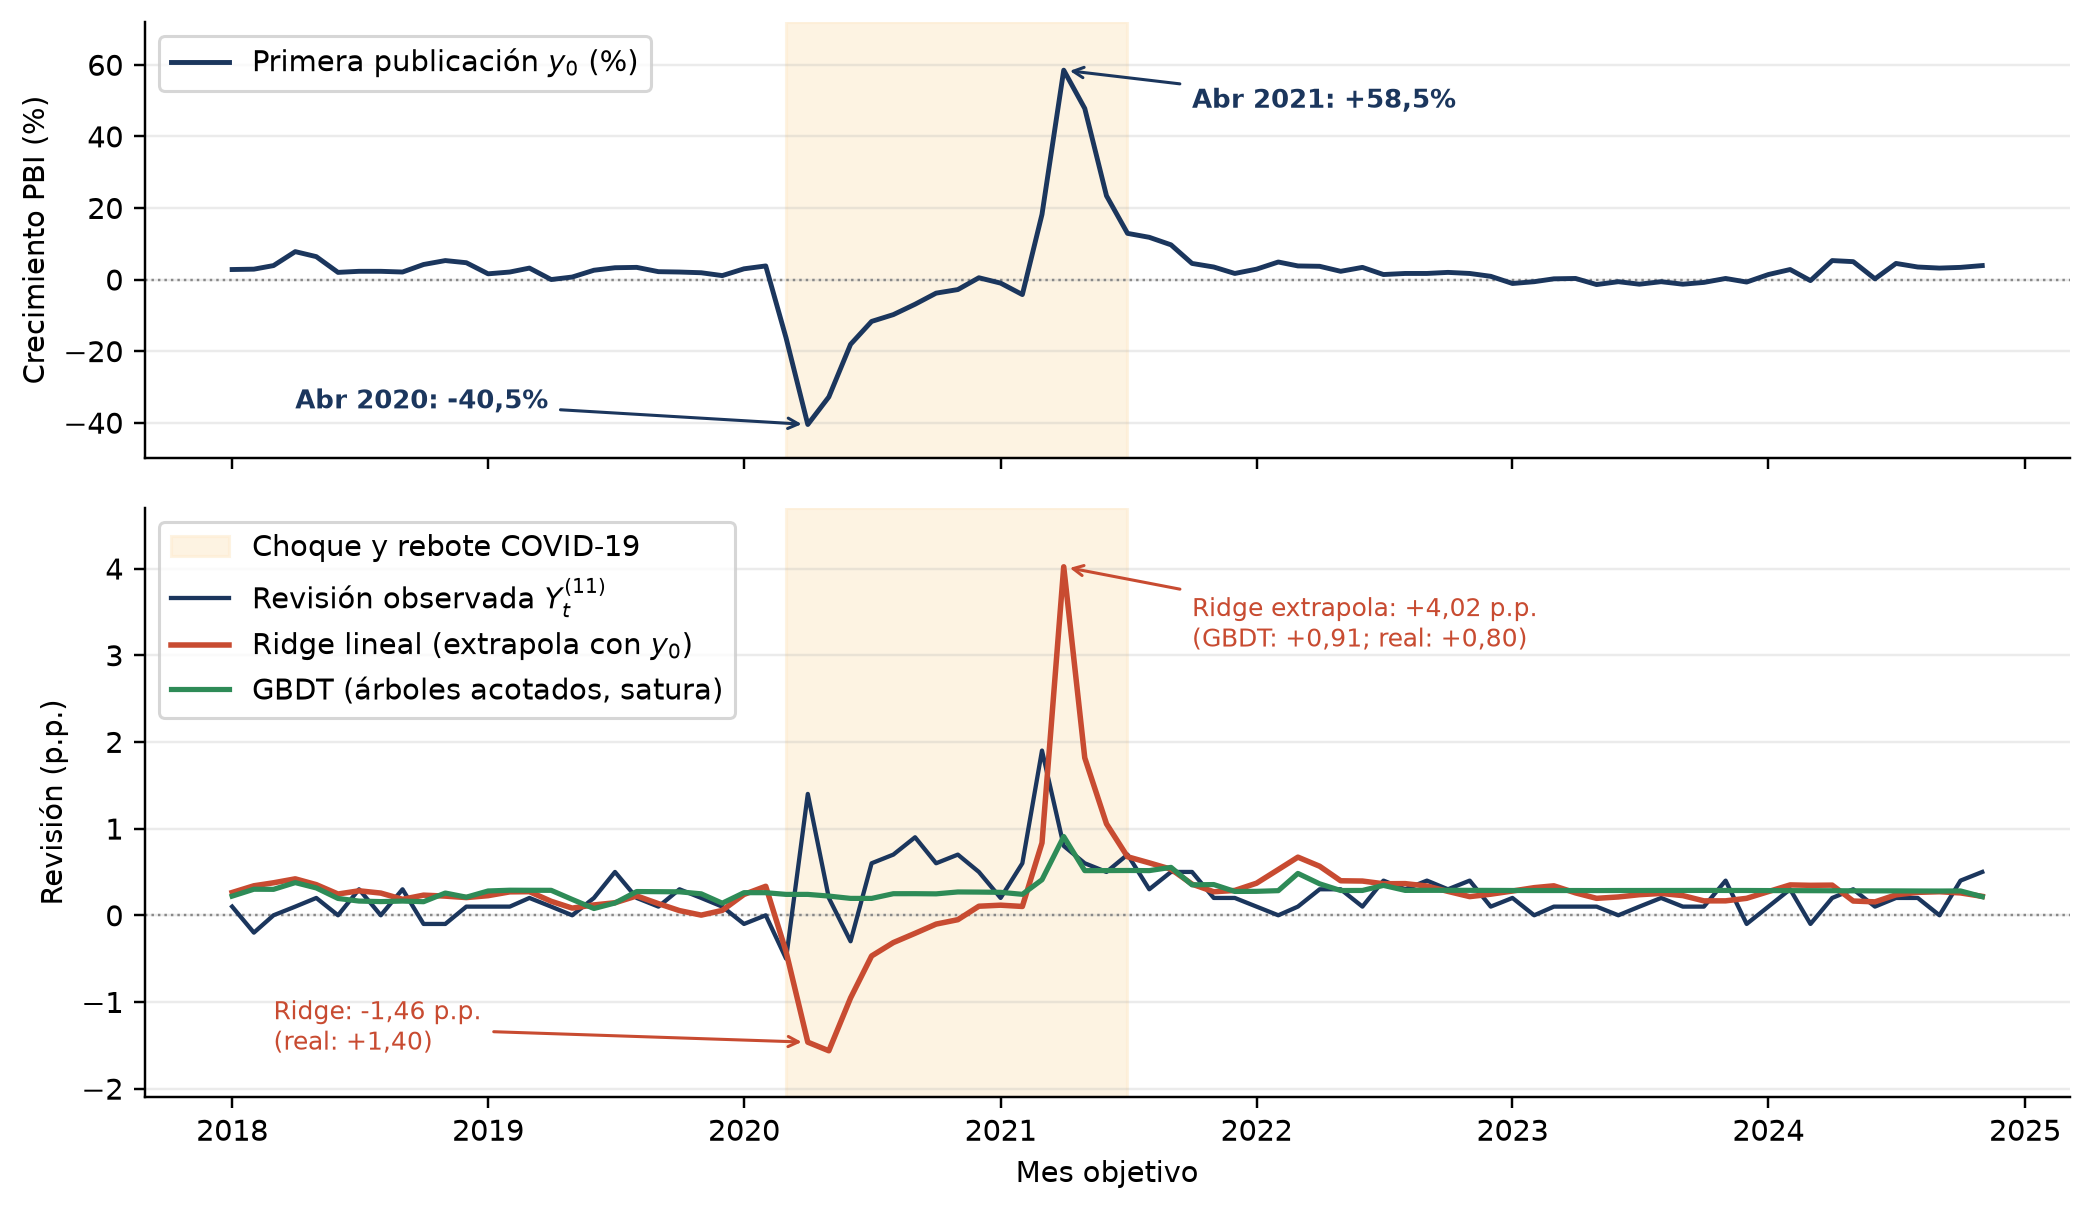
\includegraphics[width=0.93\textwidth]{figuras/fig_ridge_vs_gbdt_covid.png}
  \apanota{Construida a partir de \codigo{output/etapa3\_clasicos/etapa3\_predicciones\_oos.csv}. Muestra las predicciones de \codigo{2020m4} y \codigo{2021m4}.}
\end{figure}

¿Por qué ocurrió exactamente ese colapso? La Figura~\ref{fig:ridge_gbdt_covid} y los registros exactos de \codigo{etapa3\_predicciones\_oos.csv} lo explican sin misterio alguno. En épocas normales, el crecimiento inicial \(y_0\) oscila dentro de una banda modesta (entre \(-2\%\) y \(+10\%\)). Una ecuación lineal entrenada en ese dominio aprende una pendiente positiva moderada sobre \(y_0\) y los sectores. Cuando irrumpe el confinamiento de \textbf{abril de 2020} (\(y_0 = -40{,}5\%\), revisión real \(Y = +1{,}40\) p.p.) y un año más tarde ocurre su rebote estadístico de \textbf{abril de 2021} (\(y_0 = +58{,}5\%\), revisión real \(Y = +0{,}80\) p.p.), \textbf{toda recta extrapola indefinidamente sin freno}:
\begin{itemize}
  \item \codigo{Ridge} predijo \(-1{,}464\) p.p. en abril de 2020 y \(+4{,}020\) p.p. en abril de 2021 (¡un error de \(+3{,}22\) p.p. en un solo mes!).
  \item \codigo{DFM\_Factor\_Ridge} extrapolo todavía más lejos: \(-1{,}701\) p.p. en 2020m4 y \(+5{,}042\) p.p. en 2021m4.
  \item \codigo{ARX\_BIC} predijo \(-1{,}722\) p.p. y \(+2{,}473\) p.p., respectivamente.
\end{itemize}

Un árbol de decisión (\codigo{GBDT\_NumPy}), por el contrario, particiona el espacio mediante reglas de umbral del tipo ``¿es \(y_0 > 6{,}5\%\)?''. Para ese corte booleano, un valor extremo de \(+58{,}5\%\) cae en exactamente la misma hoja terminal acotada que un mes de auge normal de \(+8\%\). Como consecuencia, \codigo{GBDT\_NumPy} mantuvo pronósticos contenidos de \(+0{,}241\) p.p. en abril de 2020 y \(+0{,}909\) p.p. en abril de 2021, logrando el mejor desempeño del bloque congelado (\(\text{RMSE} = 0{,}349\), \(\text{MAE} = 0{,}237\), \(R^2_{\text{OOS}} = +0{,}087\)), como sintetiza la Figura~\ref{fig:rmse_regimenes}.

\begin{figure}[htbp]
  \caption{Comparación de RMSE fuera de muestra por regímenes para los ocho referentes clásicos}
  \label{fig:rmse_regimenes}
  \centering
  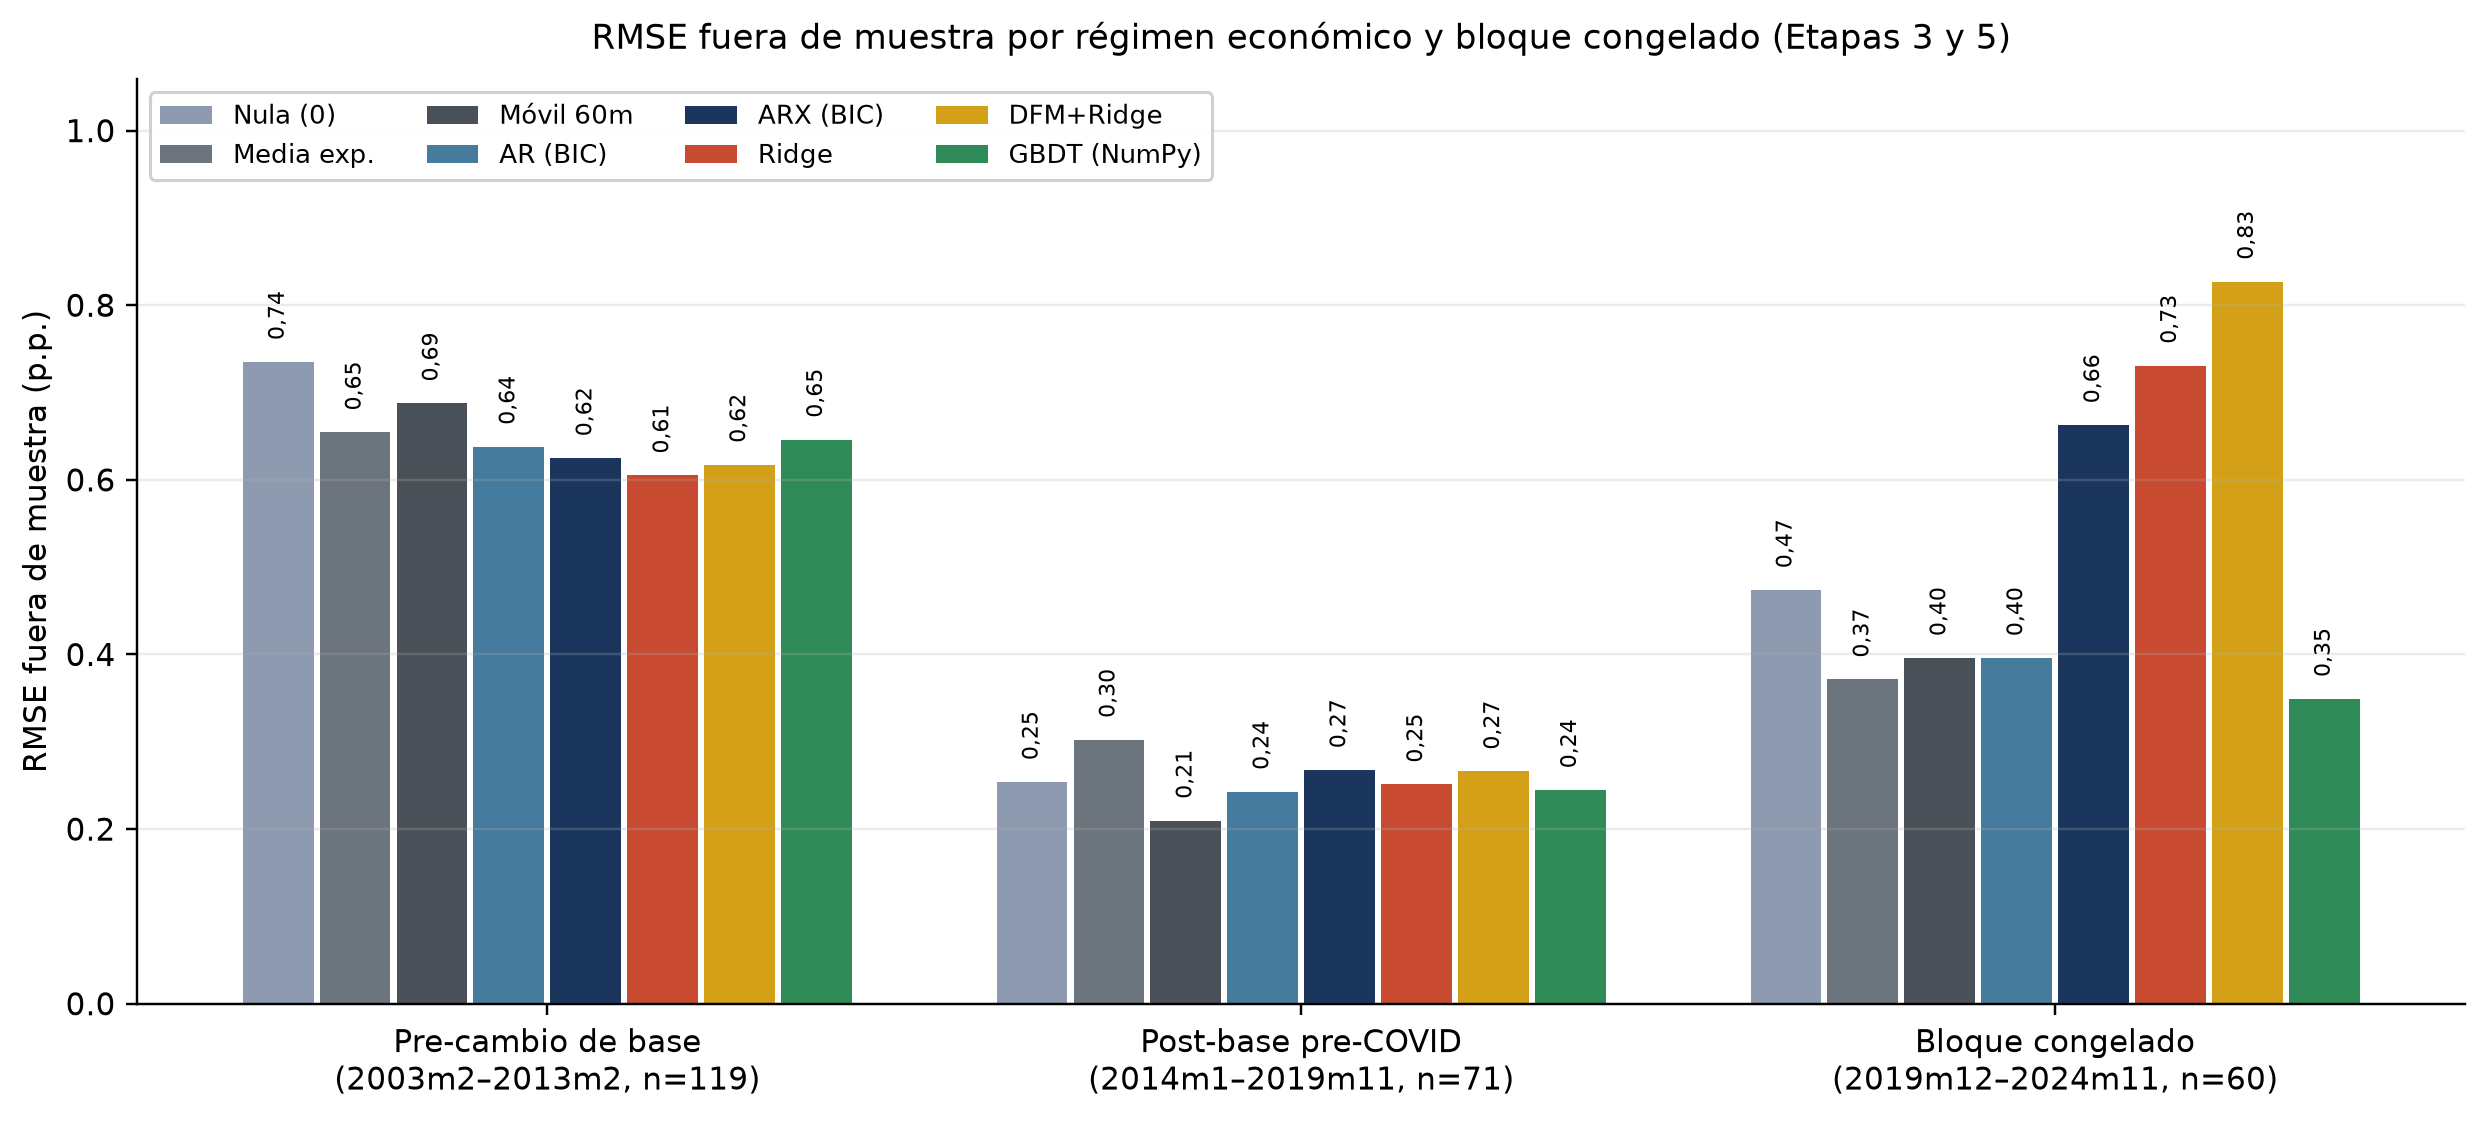
\includegraphics[width=0.94\textwidth]{figuras/etapa3_rmse_regimenes.png}
  \apanota{Tomado de \codigo{output/etapa3\_clasicos/etapa3\_rmse\_regimenes.png}. Evidencia la inversión de ranking entre tiempos regulares y el episodio pandémico.}
\end{figure}

Esta constatación deja perfectamente trazada la pregunta científica para la Etapa~4: puesto que tanto la falla de Ridge como el rechazo RESET de 2020--2024 obedecieron a la extrapolación lineal sin cotas ante choques extremos, ¿puede un reservorio no lineal suavemente acotado —clásico (ESN/RFF) o cuántico (QRC)— conservar la precisión de Ridge en años normales y evitar su colapso durante el COVID-19?

\apabibliografia

\end{document}
